\documentclass{article}
% Chinese
% \documentclass[UTF8, nofonts, mathptmx, 12pt, onecolumn]{article}
% \usepackage{xeCJK}
% \setCJKmainfont{SimSun}
\usepackage{amsmath}
\usepackage{amsfonts}
\usepackage{amssymb}
\usepackage{wasysym}
% \usepackage{ctex}
\usepackage{graphicx}
\usepackage{float}
\usepackage{geometry}
\geometry{a4paper,scale=0.8}
\usepackage{caption}
\usepackage{subcaption}
% \newcommand{\oiint}{\mathop{{\int\!\!\!\!\!\int}\mkern-21mu \bigcirc} {}}
\newcommand*{\dif}{\mathop{}\!\mathrm{d}}
\newcommand*{\md}{\mathop{}\!\mathrm{d}}
\newcommand*{\me}{\mathrm{e}}

% \usepackage{parskip}
% \setlength{\parindent}{0cm}

\usepackage{bm}
\let\Oldmathbf\mathbf
\renewcommand{\mathbf}[1]{\boldsymbol{\Oldmathbf{#1}}}
\let\eqnarray\align

\author{Xiping Hu}
\usepackage{authblk}
\author{Xiping Hu}
\affil{https://hxp.plus/}
\title{Homework for Chapter 4}

\begin{document}
\maketitle

\begin{figure}[H]
  \centering
  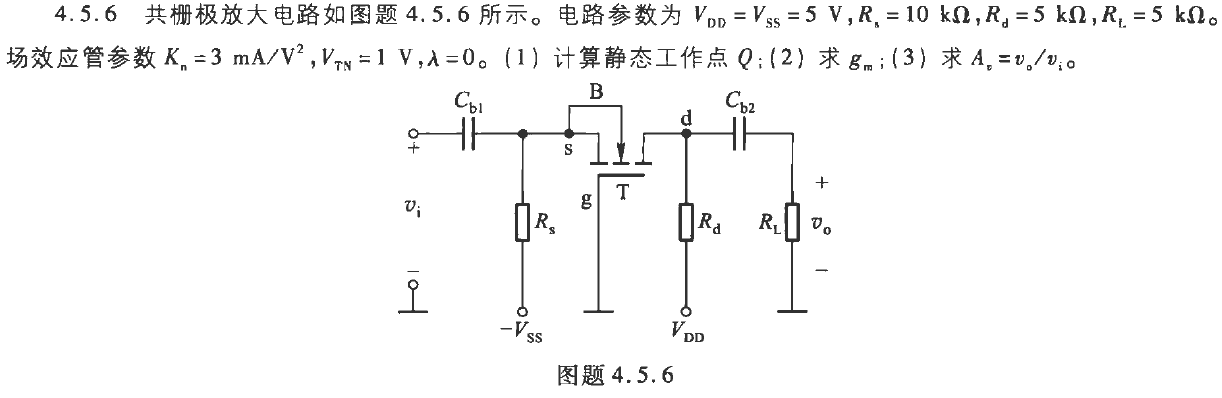
\includegraphics[width=\linewidth]{figures/Problem456}
  \label{fig:}
\end{figure}

\paragraph{Problem 1}

\begin{equation*}
  \begin{aligned}
    I_{DQ} = K_n \left( V_{GSQ} - V_{TN} \right)^2
  \end{aligned}
\end{equation*}

\begin{equation*}
  \begin{aligned}
    - V_{GSQ} - I_{DQ} R_S = - V_{SS}
  \end{aligned}
\end{equation*}

The two possible solution for $I_{DQ}$ are:

\begin{equation*}
  \begin{aligned}
    I_{DQ} = 0.438 \  \mathrm{mA}
  \end{aligned}
\end{equation*}

or

\begin{equation*}
  \begin{aligned}
    I_{DQ} = 0.365 \  \mathrm{mA}
  \end{aligned}
\end{equation*}

Noted that if $I_{DQ} = 0.438 \  \mathrm{mA}$, $V_{GSQ} = 0.62 \  \mathrm{V} < V_{TN} $. So that this solution is invalid. $I_{DQ} = 0.365 \  \mathrm{mA}$ when $V_{GSQ} = 1.35 \  \mathrm{V}$

\paragraph{Problem 2}

\begin{equation*}
  \begin{aligned}
    g_m = 2 K_n \left( V_{GSQ} - V_{TN}  \right) = 2.1 \  \mathrm{mA/V}
  \end{aligned}
\end{equation*}

\paragraph{Problem 3}

\begin{equation*}
  \begin{aligned}
    A_v = g_m \cdot \dfrac{R_d R_L}{R_d + R_L} = 5.25 
  \end{aligned}
\end{equation*}


\end{document}